\documentclass{article}

\usepackage[margin=1in]{geometry}
\usepackage{amsmath,amsthm,amssymb}
\usepackage{bbm,enumerate,mathtools,mathrsfs}
\usepackage[hidelinks]{hyperref}
\usepackage{tikz}
\usetikzlibrary{matrix, arrows}

\newenvironment{problem}[2][Problem]{\begin{trivlist}
\item[\hskip \labelsep {\bfseries #1}\hskip \labelsep {\bfseries #2.}]}{\end{trivlist}}
\newenvironment{solution}[1][Solution.]{\begin{trivlist}
\item[\hskip \labelsep {\bfseries #1}]}{\end{trivlist}}
\newenvironment{problempart}[1]{\begin{trivlist}\item[\textbf{Part #1.}]}{\end{trivlist}}

\newenvironment{definition}[1][Definition.]{
  \begin{trivlist} \item[\hskip \labelsep {\bfseries #1}]
}{\end{trivlist}}

\newenvironment{example}[1][Example.]{
  \begin{trivlist} \item[\hskip \labelsep {\bfseries #1}]
}{\end{trivlist}}

\newenvironment{note}[1][Note.]{
  \begin{trivlist} \item[\hskip \labelsep {\bfseries #1}]
}{\end{trivlist}}

\newenvironment{theorem}[1][Theorem.]{
  \begin{trivlist} \item[\hskip \labelsep {\bfseries #1}]
}{\end{trivlist}}

\newenvironment{exercise}[1][Exercise.]{
  \begin{trivlist} \item[\hskip \labelsep {\bfseries #1}]
}{\end{trivlist}}

\newcommand{\set}[1]{\{ #1 \}}
\newcommand{\ang}[1]{\langle #1 \rangle}
\newcommand{\paren}[1]{\biggl( #1 \biggr)}
\newcommand{\fn}[3]{#1 \colon #2 \rightarrow #3}

\begin{document}

\title{Algebraic Combinatorics: Homework 2}
\author{Peter Kagey}

\maketitle

% -----------------------------------------------------
% First problem
% -----------------------------------------------------
\begin{problem}{1}
  Let $f(n)$ denote the number of structures on $[n]$, and let $e(n)$ denote the
  number of such structure for which the number of components is even. Prove \[
    E(x) = \frac 12 \paren{F(x) + \frac 1{F(x)}}
  \]
\end{problem}

\begin{proof} $ $
  Let the sub-structure be denoted by $g(n)$, that is \begin{align*}
    f(\#S) &= \sum_{\set{B_1,\hdots,B_k} \in \Pi(S)} g(B_1)\cdots g(B_k) \\
    F(x) &= \exp(G(x))
  \end{align*} so that the ``even'' structure is \begin{align*}
    e(\#S) &= \sum_{\set{B_1,\hdots,B_k} \in \Pi(S)} g(B_1)\cdots g(B_k)h(k) \\
    E(x) &= H(G(x))
  \end{align*} where \[
    h(k) = \begin{cases}
      1 & k \text{ is even} \\
      0 & \text{otherwise}
    \end{cases},
  \]
  and thus \[
    H(x) = \sum_{n=0}^\infty \frac{x^{2n}}{(2n)!}
    = \cosh(x)
    = \frac 12 \paren{e^x - e^{-x}}.
  \]
  And the desired identity follows: \begin{align*}
    E(x)
    &= H(G(x)) \\
    &= \frac 12 \paren{\underbrace{\exp(G(x))}_{F(x)} - \exp(G(x))^{-1}} \\
    &= \frac 12 \paren{F(x) - F(x)^{-1}}.
  \end{align*}
\end{proof}
\pagebreak
\begin{problem}{2}
  Let $T(x)$ be the exponential generating function for threshold graphs, and
  let $S(x)$ be the exponential generating function for threshold graphs with
  no isolated vertex.
  \begin{enumerate}[(a)]
    \item Find the first four coefficients of $T(x)$ and $S(x)$.
  \end{enumerate}
\end{problem}
\begin{solution} \text{} \\
  \begin{enumerate}[(a)]
    \item \begin{alignat*}{2}
      T(x) &= 1 + x &&+ \frac{2}{2!}x^2 + \frac{8}{3!}x^3 \\
      S(x) &= 1     &&+ \frac{1}{2!}x^2 + \frac{4}{3!}x^3
    \end{alignat*}
    \item Let $t_k(n)$ be the number of threshold graphs with exactly $k$
    isolated vertices. Then
    $t_k(n) = \binom nk s(n-k)$ by choosing which $k$ vertices are isolated, and
    imposing any non-isolated vertex structure on the remaining $n-k$ vertices. \[
      t(n) = \sum_{k=0}^n t_k(n) = \sum_{k=0}^n \binom nk s(n-k).
    \]
    Notice that since the coefficients of $e^x$ are all $1$, \[
      e^xS(x) = \sum_{n=0}^\infty\paren{\underbrace{\sum_{k=0}^n \binom nk s(n-k)}_{t(n)}}\frac{x^n}{n!}
      = T(x).
    \]
    \item When $n = 0$, there is one threshold graph, and it does not have an
    isolated vertex.
    \\~\\
    When $n=1$, there is one threshold graph, and it has an isolated vertex.
    \\~\\
    When $n \geq 2$, given a threshold graph with an isolated vertex $v$,
    its complement has no isolated vertex---in particular, every vertex in the
    complement is connected to $v$. Taking the complement gives a 1-1
    correspondence between threshold graphs with an isolated vertex and
    threshold graph with no isolated vertex.
    \\~\\
    Therefore $T(x) = 2S(x) + x - 1$, where the $+x - 1$ corrects for the $n=0$
    and $n=1$ cases.
    \item Using \begin{align*}
      2S(x) + x - 1 &= T(x) = e^xS(x)\\
      2S(x) - e^xS(x) &= 1 - x \\
      S(x) &= \frac{1 - x}{2 - e^x}
    \end{align*} Then using $T(x) = e^xS(x)$ gives \[
      T(x) = e^x\frac{1 - x}{2 - e^x}.
    \]
  \end{enumerate}
\end{solution}
\pagebreak
%%%%%%%%%%%%
%
% Problem 3
%
%%%%%%%%%%%%
\begin{problem}{3}
  Let $G$ be a simple graph on $[n]$ with $k$ connected components. Prove that
  $G$ is a forest if and only if $G$ has $n - k$ edges.
\end{problem}

\begin{solution} $ $\\
  Consider the connected components of $G$, which have $n_1, n_2, \hdots, n_k$
  vertices respectively.
  $(\Longrightarrow)$ Assume that $G$ is a forest with $k$ connected components.
  \\
  Each connected component is a tree, each of which
  has  $n_i - 1$ edges. Then summing the edges gives the desired result: \begin{align*}
    (n_1 - 1) + (n_2 - 1) + \hdots + (n_k - 1)
    &= \underbrace{n_1 + n_2 + \hdots + n_k}_n \underbrace{- 1 - 1 \hdots - 1}_{-k} \\
    &= n - k
  \end{align*}
  $(\Longleftarrow)$ Assume that $G$ has $n-k$ edges. Every connected graph on
  $[m]$ has at least at least $m-1$ edges, so each connected components has
  $n_i + \ell_i$ edges where $\ell_i \geq -1$.
  Adding all of these up \begin{align*}
    (n_1 + \ell_1) + (n_2 + \ell_2) + \hdots + (n_k + \ell_k) &= n - k \\
    \ell_1 + \ell_2 + \hdots + \ell_3 &= -k
  \end{align*}
  But since each $\ell_i \geq -1$, this means that $\ell_i = 1$ for all $i$.
  Thus the connected components are trees, and $G$ is a forest.
\end{solution}
\pagebreak
%%%%%%%%%%%%
%
% Problem 4
%
%%%%%%%%%%%%
\begin{problem}{4}
  Let $g(n, e)$ denote the number of connected, simple graphs on $[n]$ with $e$
  edges.
  \begin{enumerate}[(a)]
    \item  Derive the mixed ordinary/exponential generating function \[
      \sum_{n=1}^{\infty}\sum_e g(n,e)q^e \frac{x^n}{n!}
      = \log\sum_{n=0}^{\infty} (1+q)^{\binom n2} \frac{x^n}{n!}
    \]
    \item Use the formula to compute $\sum_e g(n,e) q^e$ for all $n \leq 4$
    \item Verify by drawing all graphs in question.
  \end{enumerate}
\end{problem}

\begin{solution} \text{} \\
  \begin{enumerate}[(a)]
    \item First notice that \[
      \sum_{n=0}^{\infty} (1+q)^{\binom n2} \frac{x^n}{n!}
      = 1 + x + (1 + q) \frac{x^2}{2} + (1 + q)^3\frac{x^3}{3!} + (1 + q)^6\frac{x^4}{4!} + \hdots
    \] gives the number of (not necessarily connected) simple graphs, where $q$
    indexes the number of edges. (This is done by choosing or not choosing each
    of the $\binom n2$ edges on the labeled complete graph.)
    Then it is enough to exponentiate both sides to see that all simple graphs
    consist of connected components, so the usual $\exp(G(x)) = F(x)$ formula
    applies.
    \item
    Using the Taylor series for $
      \log(1 + x) = x - \frac 12 x^2 + \frac 13 x^3 - \frac 14 x^4 + \hdots
    $
    yields
    \begin{align*}
      \log\paren{1 + \sum_{n=1}^{\infty} (1+q)^{\binom n2} \frac{x^n}{n!}}
      &= \sum_{n=1}^{\infty} (1+q)^{\binom n2}\frac{x^n}{n!}
        - \frac 12\paren{\sum_{n=1}^{\infty} (1+q)^{\binom n2}\frac{x^n}{n!}}^2
        + \frac 13\paren{\sum_{n=1}^{\infty} (1+q)^{\binom n2}\frac{x^n}{n!}}^3
        - \hdots\\
      &= x + (1 + q) \frac{x^2}{2} + (1 + q)^3\frac{x^3}{3!} + (1 + q)^6\frac{x^4}{4!} + O(x^5) \\
      &- \frac 12 \paren{x^2 + (1+q)x^3 + \frac{(1+q)^3}{3}x^4 + \frac{(1+q)^2}{4}x^4  + O(x^5)} \\
      &+ \frac 13 \paren{x^3 + \frac 32(1+q)x^4 + O(x^5)} \\
      &- \frac 14 \paren{x^4 + O(x^5)}.
    \end{align*}
    Thus, simplifying, the first four terms (with respect to $n$) are \[
      \sum_{n=1}^{4}\sum_e g(n,e)q^e \frac{x^n}{n!} =
      x + q\frac{x^2}{2!} + (3q^2 + q^3)\frac{x^3}{3!} + (16q^3 + 15q^4 + 6q^5 + q^6)\frac{x^4}{4!}.
    \]
    \item  $ $\\
    $n = 1$:\hspace{1.53cm}$n = 2$:\hspace{1.53cm}$n = 3$:\\
    \begin{tikzpicture}[scale=2]
      \draw (0,0) grid (1,1);
      \fill (0.5, 0.5) circle (0.05);
      \node at (0.5, -0.1) {1};
    \end{tikzpicture}
    ~~
    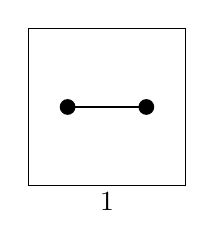
\begin{tikzpicture}[scale=2]
      \draw (0,0) grid (1,1);
      \fill
        (0.25, 0.5) circle (0.05)
        (0.75, 0.5) circle (0.05)
      ;
      \draw
        (0.25,0.5)--(0.75,0.5)
      ;
      \node at (0.5, -0.1) {1};
    \end{tikzpicture}
    ~~
    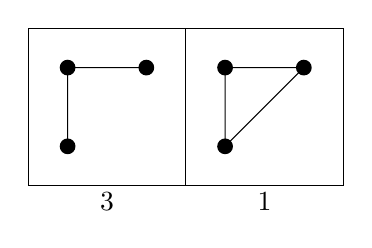
\begin{tikzpicture}[scale=2]
      \draw (0,0) grid (2,1);
      \foreach \i in {0,1} {
        \fill
          (\i + 0.25, 0.25) circle (0.05)
          (\i + 0.25, 0.75) circle (0.05)
          (\i + 0.75, 0.75) circle (0.05)
        ;
      }
      \draw
        (0.25,0.75)--(0.75,0.75) (0.25,0.75)--(0.25,0.25)
        (1.25,0.75)--(1.75,0.75)--(1.25,0.25)--cycle
      ;
      \node at (0.5, -0.1) {3};
      \node at (1.5, -0.1) {1};
    \end{tikzpicture}
    \\~\\
    $n = 4$:\\
    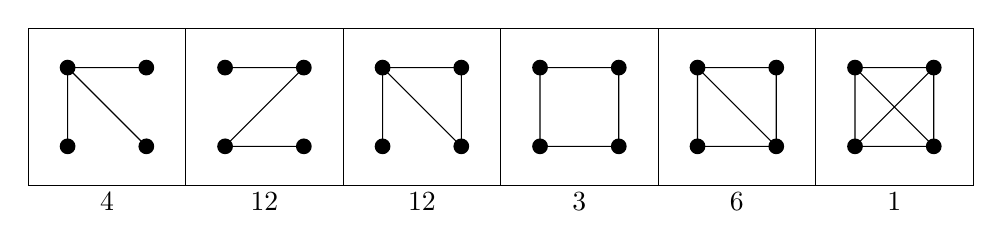
\begin{tikzpicture}[scale=2]
      \draw (0,0) grid (6,1);
      \foreach \i in {0,1,2,3,4,5} {
        \fill
          (\i + 0.25, 0.25) circle (0.05)
          (\i + 0.25, 0.75) circle (0.05)
          (\i + 0.75, 0.25) circle (0.05)
          (\i + 0.75, 0.75) circle (0.05)
        ;
      }
      \draw
        (0.25,0.75)--(0.75,0.75) (0.25,0.75)--(0.25,0.25) (0.25,0.75)--(0.75,0.25)
        (1.25,0.75)--(1.75,0.75)--(1.25,0.25)--(1.75,0.25)
        (2.25,0.75)--(2.75,0.75)--(2.75,0.25) (2.25,0.75)--(2.25,0.25) (2.25,0.75)--(2.75,0.25)
        (3.25,0.75)--(3.75,0.75)--(3.75,0.25)--(3.25,0.25)--cycle
        (4.25,0.75)--(4.75,0.75)--(4.75,0.25)--(4.25,0.25)--cycle (4.25,0.75)--(4.75,0.25)
        (5.25,0.75)--(5.75,0.75)--(5.75,0.25)--(5.25,0.25)--cycle (5.25,0.75)--(5.75,0.25) (5.75,0.75)--(5.25,0.25);
      ;
      \node at (0.5, -0.1) {4};
      \node at (1.5, -0.1) {12};
      \node at (2.5, -0.1) {12};
      \node at (3.5, -0.1) {3};
      \node at (4.5, -0.1) {6};
      \node at (5.5, -0.1) {1};
    \end{tikzpicture}
  \end{enumerate}
\end{solution}
\end{document}
